\subsection{Interoperability — what!?}\label{subsec:IntegrationVsInteroperability}
\begin{frame}{Interoperability — what!?}
  \begin{center}
    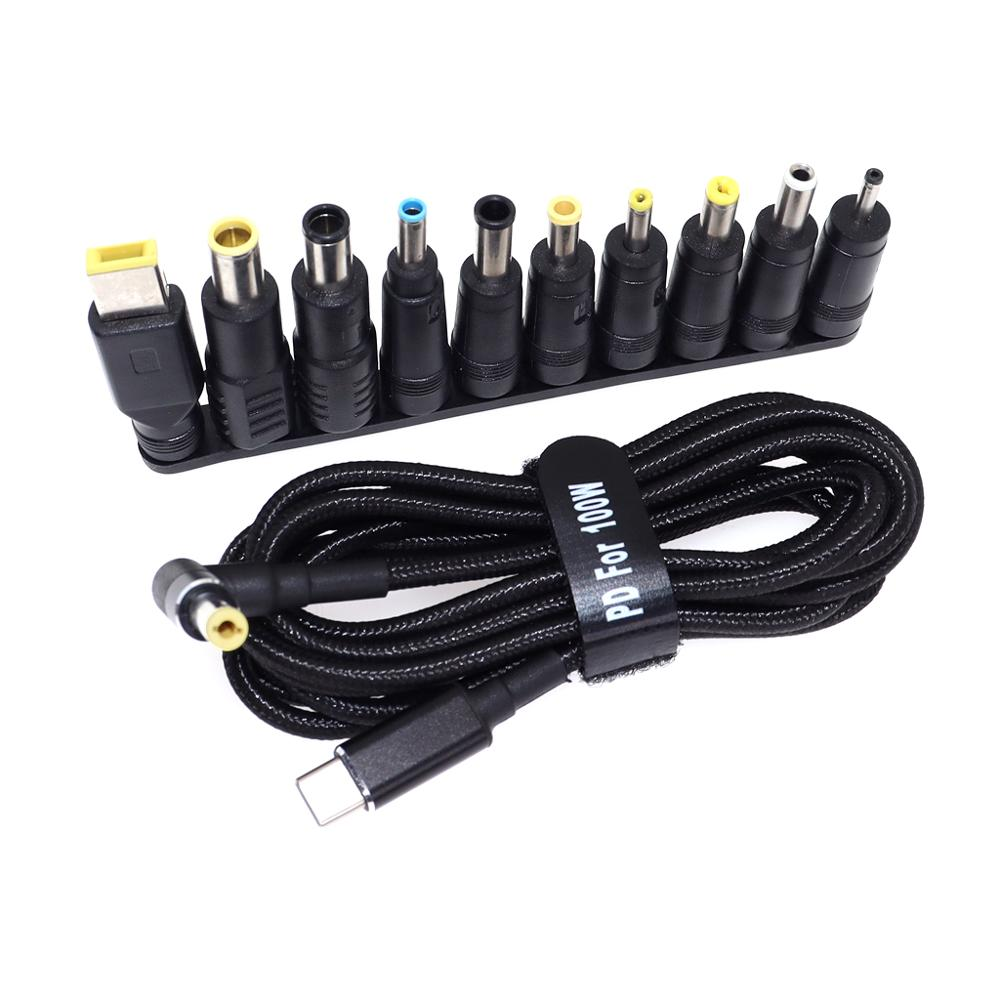
\includegraphics[height=0.32\textheight]{slides/context/cables/figs/cable-adapters.jpeg}%
    \qquad
    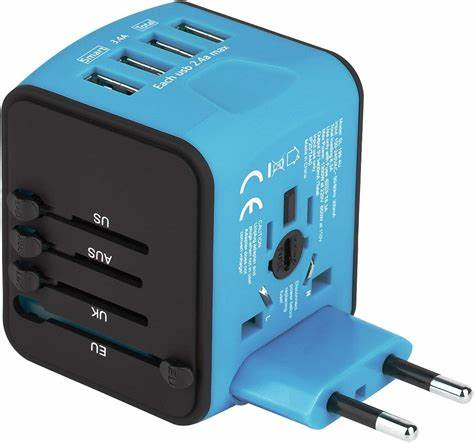
\includegraphics[height=0.32\textheight]{slides/context/cables/figs/travel-charger.jpeg}
  \end{center}

  \vspace{0.4cm}
  \begin{center}
    {\large\itshape Upon further reflection:}
  \end{center}
  \vspace{0.3cm}
  \begin{alertblock}{}
    When systems can work together but have been \emph{modified} to do so, they are \alert{integrated}.
    \vspace{0.2cm}
    \small Merriam Webster: $[\,$systems that are$\,]$ designed to work with another device or system \emph{without modification} $[\,$are compatible$\,]$.
  \end{alertblock}
\end{frame}
